\documentclass[18pt]{extarticle}

% set lengths
\setlength{\textheight}{9in}
\setlength{\textwidth}{7.1in}
\setlength{\evensidemargin}{-0.2in}
\setlength{\oddsidemargin}{-0.2in}
\setlength{\headsep}{30pt}
\setlength{\topmargin}{-0.3in}

% packages
\usepackage{amsthm}
\usepackage{hyperref}
\usepackage{amsmath}
\usepackage{amssymb}
\usepackage{qtree}
\usepackage{enumitem}
\usepackage{wasysym}
\usepackage{courier}
\usepackage{textcomp}
\usepackage{nicefrac}
\usepackage{graphicx}
\usepackage{stackengine}
\usepackage{mathtools}
\usepackage{blindtext}
\usepackage{scrextend}
\addtokomafont{labelinglabel}{\sffamily}

\def\delequal{\mathrel{\ensurestackMath{\stackon[1pt]{=}{\scriptstyle\Delta}}}}

\pagestyle{myheadings}

%%%%%%%%%%%%%%%%%%%%%%%%%%%%%%%%%%%%%%%%%%%%%%%%%%%%%%%%%%%%%%%%%%%%%%


\begin{document}


% headings aligned
CAS CS 512

Surya Vajjhala \{vajjhala \large{\textbf{@}} \small{bu.edu}\}

% Title of document
\begin{center}
\Large{\textbf{Project Report}}
\end{center}

\begin{center}
\Large{\textbf{Formal Verification and Implementation of Peterson's Algorithm for Mutual Exclusion}}
\end{center}

\section*{The Problem}
In a distributed program, a number of different components are simultaneously executed, but the critical section is only accessible to one component at a time. \newline \newline
The  problem is to find a \textit{protocol} to allow only one of the competing components access to the critical section. \newline
Peterson's mutual exclusion algorithm is one of the many algorithms that solves this problem. \newline

The properties we need to check for are:
\begin{enumerate}
\item \textbf{Safety}: Only one process is in the critical section at any time.
\item \textbf{Liveness}: Every requesting process must eventually get access to the critical section.
\end{enumerate}


\section*{Approach}

I will start with the primitive algorithm for mutual exclusion, which is the the Safe Sluice algorithm, show how it fails to address deadlock, then extract the Peterson's algorithm from the \textit{safety} condition. \newline \newline
The algorithm I will be arguing about will be a variant of the Peterson's algorithm that synchronises only two components, but the general version extends this to n components. \newline \newline
At the end of the report I have presented the pseudo-code for the \textbf{N}-component variant without proof. It is this version that I have implemented.


\section*{Notation}

The pseudo-code used Dijkstra's Guarded Command Language

\begin{labeling}{alligator}
\item [skip] does nothing
\item [x := E] Assignment of evaluated expression E to x
\item [if B0 $\rightarrow$ S0 $\|$ \ B1 $\rightarrow$ S1 fi] ``Alternative Construct" Execute S0 if B0 is \texttt{true}, execute S1 if B1 \texttt{true}; terminate only if one of the guarded conditions is satisfied
\item [do B0 $\rightarrow$ S0 $\|$ \ B1 $\rightarrow$ S1 od]``Repetitive Construct" or ``Loop", keep executing S0 or S1 as long as the corresponding guards evaluate to \texttt{true}. Terminates when both are \texttt{false}
\end{labeling}

\newpage

\section*{Safe Lock or Safe Sluice algorithm}

The idea behind the safe lock is based on the analogy with the locks that sit in dikes where boats sail in opposite direction. The captain of one boat uses a flag to signal to the other boat. The other boat will only sail when no flag is signalled.
\newline

\begin{figure}[h]
  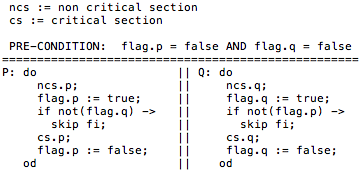
\includegraphics[scale=0.7]{safelock}
  \label{fig: safe-lock algorithm}
\end{figure}



The safe lock ensures only one component can have access to the critical section. But you can have a situation where both the \textbf{flag.p} and \textbf{flag.q} are both set to \textbf{true} and you can have a deadlock. \newline 
\section*{Extracting Peterson's}
For this reason we introduce a new condition \textsl{H.p} into the \textbf{if} statement. The idea here is to weaken the guard so that total deadlock does not occur. \newline \newline
So the current guarded \textbf{if} statement is replaced with \texttt{if not flag.q $\lor$ H.p $\rightarrow$ skip fi} \newline

Lets call the post condition after this \textbf{if} statement terminates as \textbf{A.p} \newline 

\begin{figure}[h]
  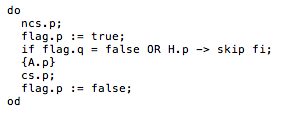
\includegraphics[scale=0.7]{2}
  \label{fig: version2}
\end{figure}

$ A.p \equiv \textsl{flag}.p \land (\neg \textsl{flag}.q \lor H.p) $ \newline

Recall that the \textit{safety} condition states that the ``Only one process is in the critical section at any time". \newline
Therefore, what we want is $\Box A.p \land A.q \Rightarrow false$, which is the strongest statement we can make about the system state. \newline

$
\begin{matrix}
        & A.p \wedge A.q \\
       \equiv & \{\mbox{definition of A}\} \\
        & \textsl{flag}.p \wedge (\neg \textsl{flag}.q \vee H.p) \wedge \textsl{flag}.q \wedge (\neg \textsl{flag}.p \vee H.q) \\
       \equiv & \{\mbox{predicate calculus}\} \\
        & \textsl{flag}.p \wedge H.p \wedge \textsl{flag}.q \wedge H.q\\
       \Rightarrow & \{\mbox{we cannot infer anything about \textsl{flag}.p or \textsl{flag}.q}\} \\
        & H.p \wedge H.q \\
       \Rightarrow & \{\mbox{which is to be proven}\} \\
        & false 
\end{matrix}
$

\newpage

Now because \textsl{H.p} occurs as a disjunct in the guard, progress is best ensured by choosing \textsl{H.p} as weak as possible, or $\neg$\textsl{H.p} as strong as possible. A choice we can make for this is to introduce a new variable \textsl{v} as the following: \newline 

$
\begin{matrix}
&\neg H.p: v=p, \ \ \ \text{or} \\
&\ \ \ \ \ H.p: v \neq p \Rightarrow v = q
\end{matrix}
$

Now by replacing this new definition into the pseudo-code, we arrive at:

\begin{figure}[h]
  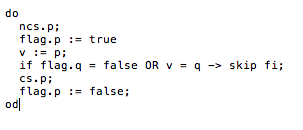
\includegraphics[scale=0.7]{3}
  \label{fig: version3}
\end{figure}

This is the Peterson's Algorithm which is  executed by each concurrent process \textsl{P}.

\section*{Check for Deadlock}
In the case of the safe lock algorithm, when both \textbf{flags} were set to \textbf{true}, we had a deadlock. \newline \newline
We now follow the order of execution dictated by the Peterson's algorithm and see  if in case both the \textbf{flags} are set to \textbf{true} whether or not we have a deadlock. \newline

\begin{align*}
      & \{\neg \text{flag}.p \wedge \neg \text{flag}.q \} \\
      & \ \ Q: v \coloneqq q \ \ \\
       & \{\neg \text{flag}.p \wedge \neg \text{flag}.q \wedge v = q\} \\
      & \ \ P: v\coloneqq p \ \ \\
      & \{\neg \text{flag}.p \wedge \neg \text{flag}.q \wedge v = p\} \\
    & \ \  P: \text{flag}.p \coloneqq true \ \ \\ 
      & \{\text{flag}.p \wedge \neg \text{flag}.q \wedge v = p\} \\
     & \ \ P: \text{if} \neg \text{flag}.q \vee v = q \rightarrow \text{skip fi} \ \ \\
      & \{\text{flag}.p \wedge \neg \text{flag}.q \wedge v = p\} \\
     & \ \ Q: \text{flag}.q \coloneqq true \ \ \\
      & \{\text{flag}.p \wedge \text{flag}.q \wedge v = p\} \\
     &\ \ P: \text{if} \neg \text{flag}.p \vee v = p \rightarrow \text{skip fi} \ \ \\
      & \{\text{flag}.p \wedge \text{flag}.q \wedge v = p\} \\
       & \ \ \ Q: cs.q      \\
\end{align*}

Thus we have shown that even though, both the \textbf{flags} are set to \textbf{true} only one of them gets access to the critical section. Thereby holding the safety condition.

\newpage

\section*{N variant of Peterson's Algorithm}

This is the pseudo-code for the N-variant of the Peterson's Algorithm  where you have N components trying to get access to the critical section. I merely state the pseudo-code here, \cite[p. ~275]{fg99} but the proof is similar to the 2 component case shown above. 
\begin{figure}[h]
  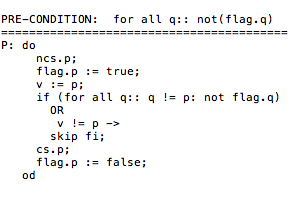
\includegraphics[scale=0.7]{4}
  \label{fig: version4}
\end{figure}

\section*{Reasoning about liveness}

Now we address liveness, which means that every system after a finite number of steps will enter the critical section. Unfortunately there is no formal liveness argument that has been published.\cite[p.~277]{fg99} And I have not made an attempt to formally prove it myself. Hence I will try to reason about it informally. \newline

Here we come back to the use of the extra variable \textsl{v} introduced. At most one component can be blocked in the guarded skip, thanks to the disjunct $\textsf{v} \neq \textsl{p}$.  Now let a component \textbf{P} be blocked indefinitely in this guarded skip. We show that within a finite number of steps the guards will become stably \textbf{true}.  \newline

There are two different computations that can be generated by the system:
\begin{enumerate}
\item Some component \textbf{Q} initiates it's \textit{repetitive construct}( \textbf{do} \{ \ \ \ \} \textbf{od} ). It will make $\textsf{v} \neq \textsl{p}$ \textbf{true} through $\textsf{v} := \textsl{q}$ - and hence component \textbf{P}'s \textit{guarded skip} will be \textbf{true}.
\item No component \textbf{Q} initiates it's \textit{repetitive construct} while component \textbf{P} is blocked. In this case the system will generate stable truth of $ \langle \forall q: q \neq p: \neg \text{flag}.q \rangle$. The argument is as follows, any component that is outside the \textit{repetitive construct} would have $\neg \text{flag}.q$ through $\text{flag}.q := \text{false}$ which is set  before finishing the program fragment.
\end{enumerate}

Through this informal argument liveness is guaranteed. \newline

We have now show that both \textit{safety} and \textit{liveness} are guaranteed by the Peterson's mutual exclusion algorithm.\newpage

\section*{Transition System for the two component case}

Instead of \textsl{flag.p} and \textsl{flag.q} I will be using \textsl{x.p} and \textsl{x.q} respectively. 

There are three variables in question here, which determine the state, \textsl{x.p}, \textsl{x.q} and \textsl{v}. \textsl{cs.p}
 refers to \textsl{P} being in the critical system and \textsl{cs.q} refers to \textsl{Q} being in the transition system. \newline
 
 From the transition system we can reason about safety and liveness\cite{lcs}:
 \begin{enumerate}
 \item \textbf{Safety}: $\Box \neg(\text{cs.p} \land \text{cs.q})$ : We can see that there is no state where both \textsl{cs.p} and \textsl{cs.q} are satisfied.
 \item \textbf{Liveness}: The liveness of component \textbf{P} is expressed as $\Box \ \text{x.p} \rightarrow \Diamond  \ \text{cs.p} $. We can see that starting at state $s_0$, when \textsl{x.p} is \textsl{true}, we reach state $s_1$ and from here both the possible paths lead to \textsl{cs.p} via paths $s_1 \rightarrow s_2$ or $s_1 \rightarrow s_3 \rightarrow s_4 \rightarrow s_5$
Even when we take the path $s_0 \rightarrow s_6$ , we will eventually reach $s_0$ or $s_1$ and hence we can again satisfy the liveness of component\textbf{P}.
Symmetrically we can reason about component \textbf{Q} as well. \newline
 \end{enumerate}
 
\begin{figure}[h]
  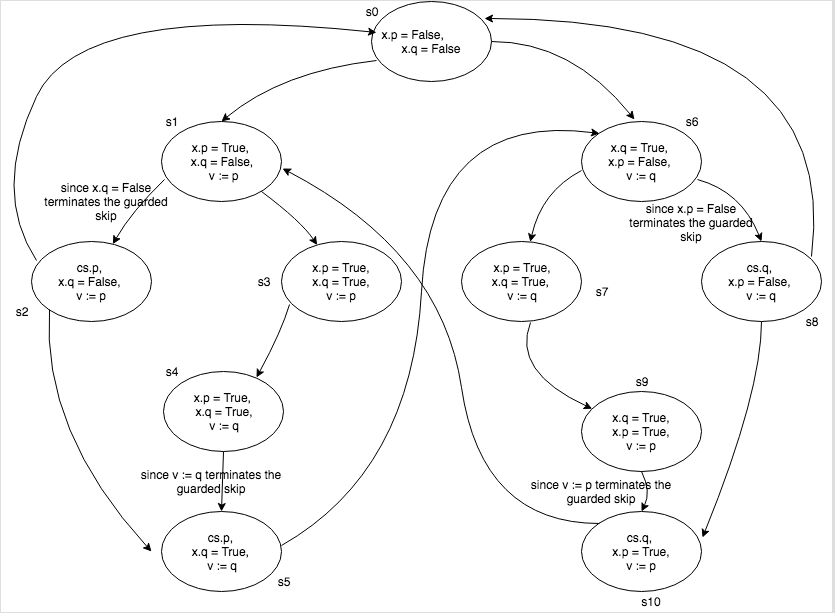
\includegraphics[scale=0.6]{tss}
  \label{fig: Transition System}
\end{figure} 
\newpage

\section*{Implementation Details}
 In this section I will discuss various details about my implementation and then mention the test cases along with the outputs.
 \subsection*{GCL to Python3}
 There are two main constructs in GCL, the "Alternate Construct" and the "Repetitive Construct".
 \begin{enumerate}
 \item \textbf{Alternate Construct}: \textbf{if B0 $\rightarrow$ S0 $\|$ \ B1 $\rightarrow$ S1 fi}
 \begin{figure*}[h]
  \centering
  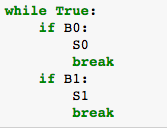
\includegraphics[scale=0.6]{ac}
  \label{fig:  if-fi}
 \caption{Python 3 implementation of Alternate Construct}
\end{figure*}
\item \textbf{Repetitive Construct} \textbf{do B0 $\rightarrow$ S0 $\|$ \ B1 $\rightarrow$ S1 od}
\begin{figure*}[h]
  \centering
  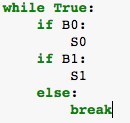
\includegraphics[scale=0.7]{rc}
  \label{fig:  do-od}
 \caption{Python 3 implementation of Repetitive Construct}
\end{figure*}
\end{enumerate}

\subsection*{Implementation} 
The base class called \texttt{Component} implements an abstract class with methods that the all the subclasses must implement. The file \texttt{petersons.py} contains it. In each of the test classes, a component is defined as an instance of a sub class of \texttt{Component}. The method \texttt{peterson} implemented by each component is run on a separate thread. \newline
 Two test cases we investigated. 
\begin{enumerate}
 \item Test Case 1, implemented in \texttt{test1.py}. Here each component is trying to modify a shared variable, by re-assigning a new value to it. 
 \item Test Case 2, implemented in \texttt{test2.py}. Here each component is trying to mutate a shared python \texttt{list}, by adding and removing elements from it. 
 \end{enumerate}
 
 Further details about the implementation are provided as in-line comments in the scripts.

\subsection*{Run}
No external libraries, so any machine with \texttt{Python 3} installed should be able to run the scripts.  \newline
To run \texttt{test1.py}: \texttt{python3 test1.py} \newline
To run \texttt{test2.py}: \texttt{python3 test2.py} \newline
Sample outputs are provided in the ``outputs" folder.


\newpage
\subsection*{Test Case 1: Change Variable}
 Three components called \texttt{s}, \texttt{p} and \texttt{q} are defined. Each tries to re-asign a new value to a shared variable. \newline
 You can see that when any component is in the critical section, either the flags of the other components are \texttt{False} or the \texttt{disjunct} is not equal to the component in the critical section. This shows that both guards in the guarded skip, \textit{alternate construct} are held. The \texttt{disjunct} is the variable \textsl{v} in the psuedo-code.
\begin{figure}[h]
  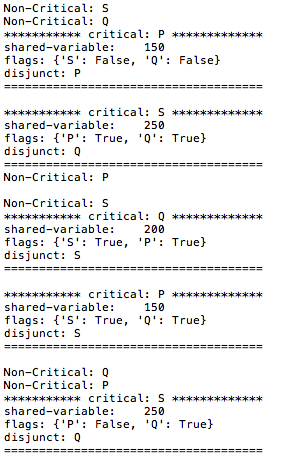
\includegraphics[scale=0.7]{t1}
  \label{fig:  }
 \caption{Sample Output for test1.py}
\end{figure}

\newpage
\subsection*{Test Case 2: Mutate a list}
Three components called \texttt{s}, \texttt{p} and \texttt{q} are defined. Each tries to mutate a shared list through appending or removing elements from the list.
Similar to the previous test case it can be verified that the guarded skip conditions are satisfied within the critical section of each component.

 \begin{figure}[h]
  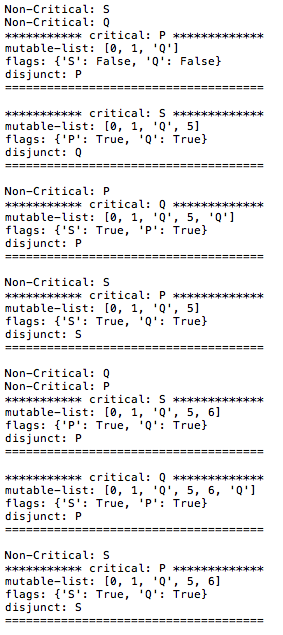
\includegraphics[scale=0.7]{t2}
  \label{fig:}
 \caption{Sample Output for test2.py}
\end{figure}


\begin{thebibliography}{9}
\bibitem{fg99}
  WHJ Feijen and AJM van Gasteren,
  Monographs in Computer Science, On a method of multiprogramming.
\bibitem{lcs}
  Michael Huth and Mark Ryan, 
  Logic in Computer Science: Modelling and Reasoning about Systems.
\end{thebibliography}


\end{document}























